%!TEX TS-program = lualatex
%!TEX encoding = UTF-8 Unicode

\documentclass[final,hyperref={pdfpagelabels=false}]{beamer}
% Width and height in cm
\usepackage[size=custom, width=111.7, height=91.4, orientation=landscape, debug, scale=1.4]{beamerposter}

%\usepackage{graphicx}
%	\graphicspath{{img/}}

	
\usepackage{fontspec}
\def\mainfont{Linux Biolinum O}
\setmainfont[Ligatures={Common,TeX}, Contextuals={NoAlternate}, BoldFont={* Bold}, ItalicFont={* Italic}, Numbers={OldStyle}]{\mainfont}
\setsansfont[Ligatures={Common,TeX}, Scale=MatchLowercase, Numbers=OldStyle]{Linux Biolinum O} 
\usepackage{microtype}

\usepackage{unicode-math}
%\setmathfont[Scale=MatchLowercase]{Tex Gyre Pagella Math}
%\setmathfont[Scale=MatchLowercase]{Asana Math}
%\setmathfont[Scale=MatchLowercase]{XITS Math}

%\usepackage[absolute,overlay]{textpos}


\usepackage{natbib}
%\setlength{\leftmargini}{0.9em}

\settowidth{\leftmargini}{\usebeamertemplate{itemize item}}
\addtolength{\leftmargini}{\labelsep}

\AtBeginDocument{%
	\abovedisplayskip=12pt plus 3pt minus 9pt
	\abovedisplayshortskip=-0.5\baselineskip
	\belowdisplayskip=12pt plus 3pt minus 9pt
	\belowdisplayshortskip=0.5\baselineskip
}
\newcommand{\whitespace}{\vspace{0.5\baselineskip}}

\mode<presentation>{
	\usetheme{SEMO}
}

% This idea from the Jacobs landscape poster template 
% http://www.latextemplates.com/cat/conference-posters
\newlength{\sepwid}
\newlength{\onecolwid}
\newlength{\twocolwid}
\newlength{\threecolwid}
\setlength{\sepwid}{0.015\paperwidth} % Separation width (white space) between columns
\setlength{\onecolwid}{0.23\paperwidth} % Width of one column
\setlength{\twocolwid}{0.464\paperwidth} % Width of two columns
\setlength{\threecolwid}{0.7\paperwidth} % Width of three columns


%%%%%%%%%%%%%%%%%%%%%%%%%%%%%%%%%%%%%%%%%%%%%%%%%%%%%%%%%%%%%%%%%%%%%%%%%%%%%%%%%5
\graphicspath{{img/}}
\title[A Quantitative Biology Curriculum]{Through the Years: A Quantitative Biology Curriculum}
\author[Taylor]{Michael S. Taylor}
\institute[SEMO]{Department of Biology}
\date{23 July 2017}


%%%%%%%%%%%%%%%%%%%%%%%%%%%%%%%%%%%%%%%%%%%%%%%%%%%%%%%%%%%%%%%%%%%%%%%%%%%%%%%%%5
\begin{document}

% To cite the Vision and Change document.
\defcitealias{national2003bio2010}{\textsc{nrc}, 2003}
\defcitealias{american2011vision}{\textsc{aaas}, 2011}

\begin{frame}[t]
%\vspace{\sepwid}
\begin{columns}[t]
	\begin{column}{\sepwid} % Left spacer
	\end{column}

	\begin{column}{\onecolwid}
    	\begin{block}{Introduction}
    		\textsc{Quantitative reasoning} is a skill that must be mastered by biology students before they graduate \citetext{\citetalias{national2003bio2010}; \citetalias{american2011vision}; \citealp{hurney2011closing}}. Yet, experience suggests that biology students do not always see the need for this skill (“I just want to work with plants.”) or fear analytical problems (“I am not good at math.”). Student aversion to quantitative analysis poses pedagogical problems for teaching the process of science.
    		
    		\whitespace

			To address these problems, some biology faculty at Southeast have coordinated to teach skills that are built upon across the curriculum. For example, the first  biology course for majors uses Microsoft Excel extensively to teach fundamental graphing and math functions for data analysis. Later courses require students to employ those early skills and to learn more advanced skills and new software such as R for simulations and analyses.  \textcolor{cardiac}{Here, I feature exercises from three courses that span the curriculum of a typical organismal biology student at Southeast.}  
    	\end{block}

		\vspace*{\sepwid}

		\begin{block}{Literature Cited}
			\setlength{\bibhang}{0.5em}
			\bibliographystyle{amnatnat}
			\raggedright
			{\small \bibliography{modeling_workshop}}
		\end{block}

		\vspace*{0.35\sepwid}

		Special thanks to Jenn Weber and Rebecka Brasso, Southeast Missouri State University.		
%		\textcolor{river}{\textbf{\textsc{Colophon}}}

		\vspace*{0.35\sepwid}

			{\justifying\small This poster was typeset with \LaTeX{} and the beamerposter package by Philippe Dreuw and Thomas Deselaers. The font is Linux Biolinum O produced by LinuxLibertine.org. The poster and template are available from mtaylor-semo on github.com  (\textsc{cc by-sa 4.0}).}

	\end{column}

	\begin{column}{\sepwid}

	\end{column}
	\begin{column}{\onecolwid}
	    \begin{block}{Year 1: Evolution and Ecology}
    	   	\textsc{Evolution and Ecology} is a new lecture and laboratory course for freshmen majors. The lab emphasizes course concepts via quantitative exercises. Specifically, students learn how to use  Excel for basic calculations and graphical analyses of real and simulated data.
			
			\whitespace
			
			\textcolor{cardiac}{\textsc{Hardy-Weinberg Equilibrium}}
			
			Students use two equations to model allele and genotype frequencies in a population. The equation for the frequencies of two alleles $\left(p \text{ and } q\right)$ is
			
			\begin{equation*}
				p + q = 1,
			\end{equation*}
			
		 	and the equation for the three possible genotypes is
			
			\begin{equation*}
				p^2 + 2pq + q^2 = 1.
			\end{equation*}
						
			Students build formulas in Excel to generate values for the five variables from $p = 0.01$ to $1.0$ and plot the three genotype frequencies (Fig.~\ref{fig:hwe}).
			
			\vspace*{0.5\baselineskip}
			
			\begin{figure}
				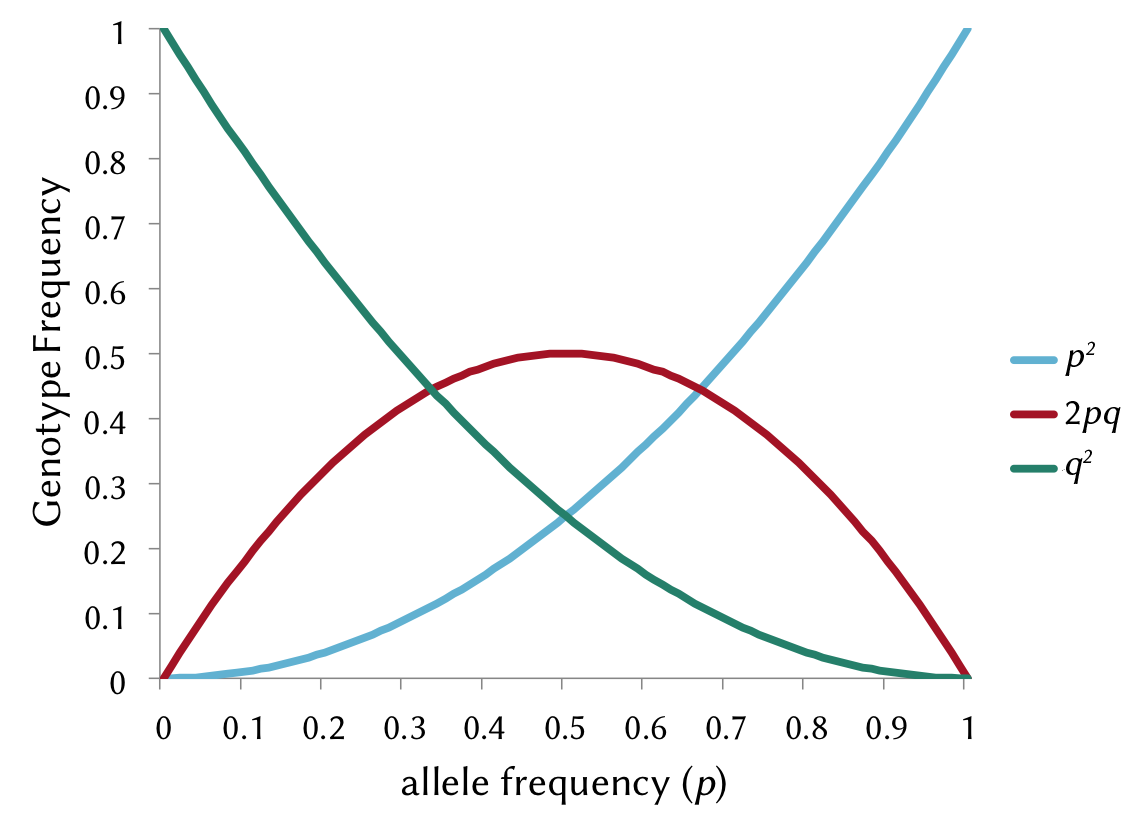
\includegraphics[width=\textwidth]{hwe_graph}
				\caption{Expected genotype frequencies for the \textit{p} allele frequency for a population in Hardy-Weinberg equilibrium.\label{fig:hwe}}
			\end{figure}
			
			\vspace*{\baselineskip}
			
			Students next apply “beanbag” biology \citep{jungck2010mathematical} by sampling “alleles” from a “population” with known allele frequencies, and then apply a $\chi^2$ test to compare observed to expected genotype frequencies. Students also explore how migration and natural selection affect allele frequencies in a population.
			
			\whitespace
			
			Representative questions from the migration component are
			
			\begin{itemize}\justifying
				\item Predict how the frequency of each allele will change for each population due to gene  flow.
				
				\item Use the results of your migration simulation to explain why gene flow between populations should prevent them from becoming genetically different.
			\end{itemize}
			
    	\end{block}
	\end{column}

	\begin{column}{\sepwid}
	\end{column}

	\begin{column}{\onecolwid}
    	\begin{block}{Years 2–3: Evolutionary Biology}
       		\textsc{Introduction to Evolutionary Biology} is taken by sophomores and juniors. The course now is lecture-only but is being redesigned to include a once-per-week lab that reinforces lecture concepts through analyses of real-world data.
       		
       		\whitespace
       		
       		\textcolor{cardiac}{\textsc{Population Genetics}}
       		
       		Students use PopG software \citep{Felsenstein2016:popg} to simulate allele frequencies in a population subject to different evolutionary scenarios such as natural selection and genetic drift. With PopG, students change population size, strength of selection, and migration and mutation rates to learn how these affect allele frequencies over time.
       		
       		\whitespace
       		
       		In one exercise, students explore the interaction between the strength of selection $\left(s\right)$ and the effective population size $\left(N_e\right)$. 
       		If $2N_es \gg 1$ then selection has a better chance of overcoming drift to cause a beneficial mutation to become fixed in the population. In  simulations where $2N_es = 0$ and $2N_es = 2$, students see that drift has the greatest effect in the first scenario but a beneficial mutation in the second scenario has about a $4\times$ greater chance of becoming fixed in the population (Fig.~\ref{fig:simulation}). 
       		
       		\vspace*{0.5\baselineskip}
       		
			\begin{figure}
			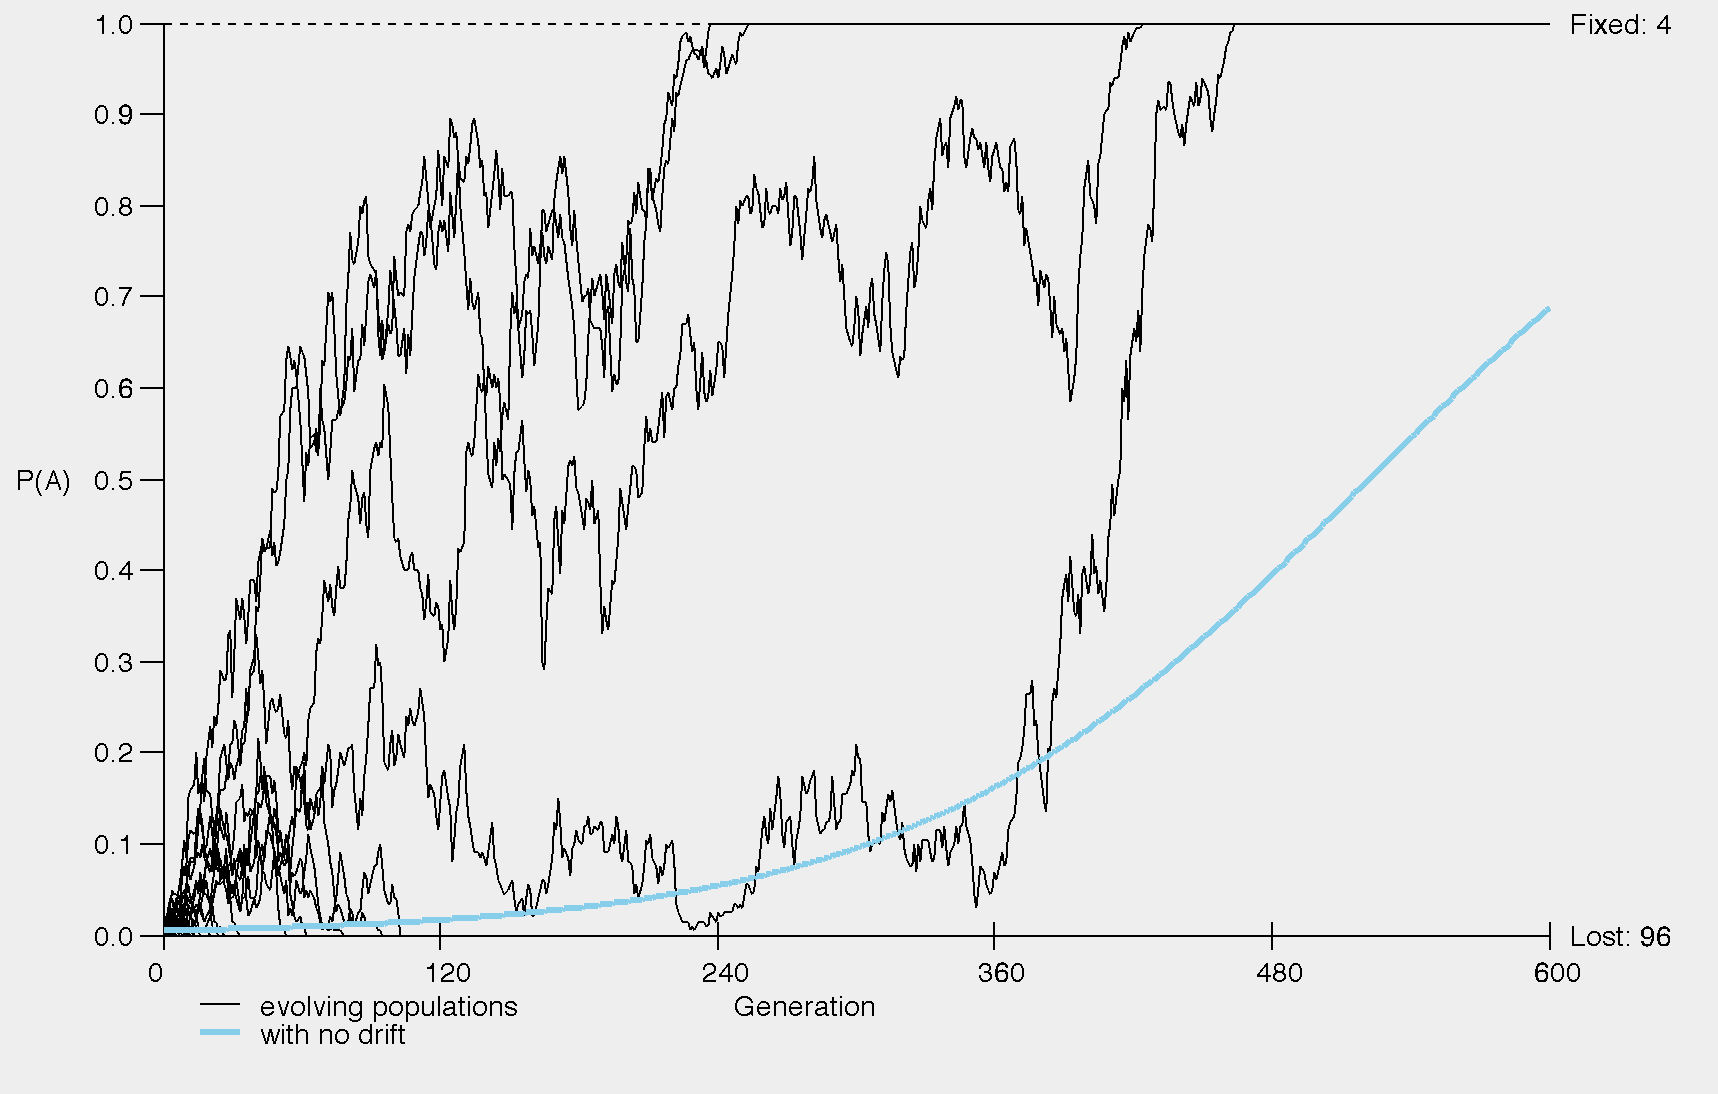
\includegraphics[width=\textwidth]{ns_graph}
			\caption{Simulation results for 100 populations with 100 individuals in each population and $s = 0.01$. The blue line represents a population without genetic drift.\label{fig:simulation}}
			\end{figure}
       		
       		\vspace*{0.8\baselineskip}
       		
       		Representative questions from this exercise are
       		\begin{itemize}\justifying
       			
       			\item Predict how $N_e$ affects the probability of fixation for an allele under weak positive selection $\left(s = 0.01\right)$. Justify your predictions for populations of $N = 1000$ and $N = 10,000$.
       			
       			\item What should be the strength of selection in a population of $N_e = 1000$ to overcome the effects of genetic drift? If $N_e = 10,000$ or $50,000$? Show your work.
       		\end{itemize}
       		
		\end{block}
	\end{column}

	\begin{column}{\sepwid}
	\end{column}

	\begin{column}{\onecolwid}
  	  	\begin{block}{Year 4: Biogeography}
			\textsc{Biogeography} is a senior and graduate level course. Students use the R Statistical Package \citep{R-Core-Team:2016aa} to analyze real-world data to discover and report biogeographic patterns.
			
       		\whitespace
       		
			\textcolor{cardiac}{\textsc{Biogeographic Provinces}}

			Students compare distribution patterns of freshwater fishes and crayfishes by performing a principal coordinates ordination (\textsc{pco}) for each taxononic group. Watersheds with shared species occur together in ordinated space (Fig.~\ref{fig:pco}).
		
			\begin{figure}
				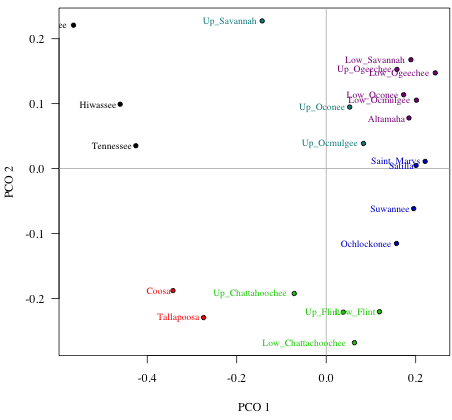
\includegraphics[width=0.94\textwidth]{fishes_pco}
				\caption{First two axes from a \textsc{pco} of Georgia fishes. Colors indicate watersheds with a similar fauna.\label{fig:pco}}
			\end{figure}
			
			Students compare fish and crayfish ordinations with a Procrustes analysis. A significant result suggests that fishes and crayfishes share a common biogeographic history (Fig.~\ref{fig:procrustes}). 
			
			\begin{figure}
				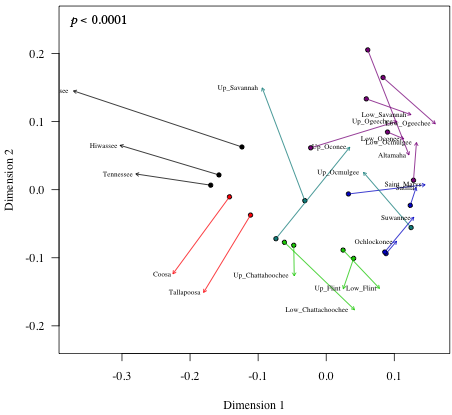
\includegraphics[width=0.94\textwidth]{procrustes}
				\caption{Procrustes analysis of fish and crayfish \textsc{pco}s. The watersheds have a  similar spatial relationships.\label{fig:procrustes}}
			\end{figure}
			
		\end{block}
	\end{column}

	\begin{column}{\sepwid}
	\end{column}

	\end{columns}
\end{frame}
\end{document}


%%%%%%%%%%%%%%%%%%%%%%%%%%%%%%%%%%%%%%%%%%%%%%%%%%%%%%%%%%%%%%%%%%%%%%%%%%%%%%%%%%%%%%%%%%%%%%%%%%%%
%%% Local Variables: 
%%% mode: latex
%%% TeX-PDF-mode: t
%%% End:
